\section{Introducing ``control''}
\subsection{}

\begin{frame}
\frametitleTC{The word ``control'' in the Merriam-Webster dictionary$^*$
              \blfootnote{\small{$^*$\texttt{https://www.merriam-webster.com/dictionary/control}}}}
\framesubtitleTC{(1/3) verb} 
\myPause
\emph{transitive verb}
\begin{tabular}{lll}
 \bf{1} & \bf{a} & archaic: to check, test, or verify by evidence or experiments \\
        & \bf{b} & :to incorporate suitable controls in \\
        &        & \textbf{//} \emph{a controlled experiment} \\
 \bf{2} & \bf{a} & :to exercise restraining or directing influence over: REGULATE \\
        &        & \textbf{//} \emph{control one's anger} \\
        & \bf{b} & :to have power over: RULE \\
        &        & \textbf{//} \emph{A single company controls the industry.} \\
        & \bf{c} & :to reduce the incidence or severity of especially to innocuous levels \\
        &        & \textbf{//} \emph{control an insect population} \\
        &        & \textbf{//} \emph{control a disease} \\
\end{tabular}\\
\vspace{2mm}\emph{intransitive verb}\\
\begin{tabular}{lll}
 :to incorporate controls in an experiment or study -- used with for \\
 \textbf{//} \emph{control for socioeconomic differences}\\
\end{tabular}
\end{frame}

\begin{frame}
\frametitleTC{The word ``control'' in the Merriam-Webster dictionary}
\framesubtitleTC{(2/3) noun} 
\myPause
\begin{tabular}{lll}
 \bf{1} & \bf{a} & :an act or instance of controlling \\
        &        & also: power or authority to guide or manage \\
        &        & \textbf{//} \emph{He took control of the family business.} \\
        & \bf{b} & :skill in the use of a tool, instrument, technique, or artistic medium \\
        &        & \textbf{//} \emph{a singer's control of her voice} \\
        & \bf{c} & :the regulation of economic activity especially by government directive \\
        &        & -- usually used in plural \\
        &        & \textbf{//} \emph{price controls} \\
        &        & \textbf{//} \emph{rent controls} \\
        & \bf{d} & :the ability of a baseball pitcher to control the location of a pitch \\
        &        & within the strike zone \\
 \bf{2} &        & :RESTRAINT, RESERVE \\
        &        & \textbf{//} \emph{exercised control of his passions}
\end{tabular}
\end{frame}

\begin{frame}
\frametitleTC{The word ``control'' in the Merriam-Webster dictionary}
\framesubtitleTC{(3/3) noun, cont'd} 
\myPause
\begin{tabular}{lll}
 \bf{3} & \multicolumn{2}{l}{:one that controls: such as} \\
        & \bf{a} & \textbf{(1)} :an experiment in which the subjects are treated as in a parallel \\
        &        &  experiment except for omission of the procedure or agent under test and which \\
        &        &  is used as a standard of comparison in judging experimental effects\vspace{1mm} \\
        &        & -- called also \emph{control experiment} \\
        &        & \textbf{(2)} :one (such as an organism, culture, or group) that is part of a control \\
        & \bf{b} & a device or mechanism used to regulate or guide the operation of a machine,\\
        &        & apparatus, or system \\
        &        & \textbf{//} \emph{the controls of the aircraft} \\
        & \bf{c} & an organization that directs a spaceflight \\
        &        & \textbf{//} \emph{mission control} \\
        & \bf{d} & a personality or spirit believed to actuate the utterances or\\
        &        & performances of a spiritualist medium \\
 \bf{4} & \multicolumn{2}{l}{or less commonly Control: CONTROL KEY}
\end{tabular}
\end{frame}

\begin{frame}
\frametitleTC{The word is prone to being misunderstood}
\framesubtitleTC{Just a couple of examples} 
\myPause
\begin{itemize}[<+-| alert@+>]
\item Many synonyms (most dangerous ones for us in bold):
      \begin{itemize}
      \item[] bridle, \textbf{check}, constrain, contain, curb, govern, hold, inhibit, \\
              keep, \textbf{measure}, pull in, regulate, rein (in), restrain,\\
              rule, tame,...
      \end{itemize}
\item Many meanings depending on the viewpoint.
\item[] \vspace{-1.5mm}For example, the controls of an aircraft ``regulate or guide'' its operation.
\item[] \vspace{-0.75mm}Fine. So what kind of object/entity do we mean here for ``controls''?
      \begin{itemize}
      \item The knobs, levers and so forth that the pilot manoeuvres?
      \item ...or the autopilot computer with its software?
      \item ...or the ailerons, the rudder and the like?
      \item ...or the compound of all of these?
      \end{itemize}
      \myPause
\item \vfill We definitely need to state our terminology and notation precisely.
\end{itemize}
\end{frame}


\begin{frame}
\frametitleTC{Our definition}
\framesubtitleTC{Take 1 -- for now mostly intuitive, we shall be progressively more precise} 
\myPause
\begin{quote}
 \begin{center}
  \Large{Control is making something behave\\
         as close as possible to how you want it to behave,\\ \myPause
         most often despite there can be other actions besides yours,\\ \myPause
         and also despite you have only a partial knowledge\\
         of the phenomena you are acting upon, \\ \myPause
         hence even the effect of your own actions\\
         may be not entirely predictable.}
 \end{center}
\end{quote}
\end{frame}

\begin{frame}\mccz
\frametitleTC{Why a \underline{theory} for systems and control?}
\framesubtitleTC{} 
\myPause
\begin{quote}
 \begin{center}
  \only<2 | handout:0>{\vspace{-0.4mm}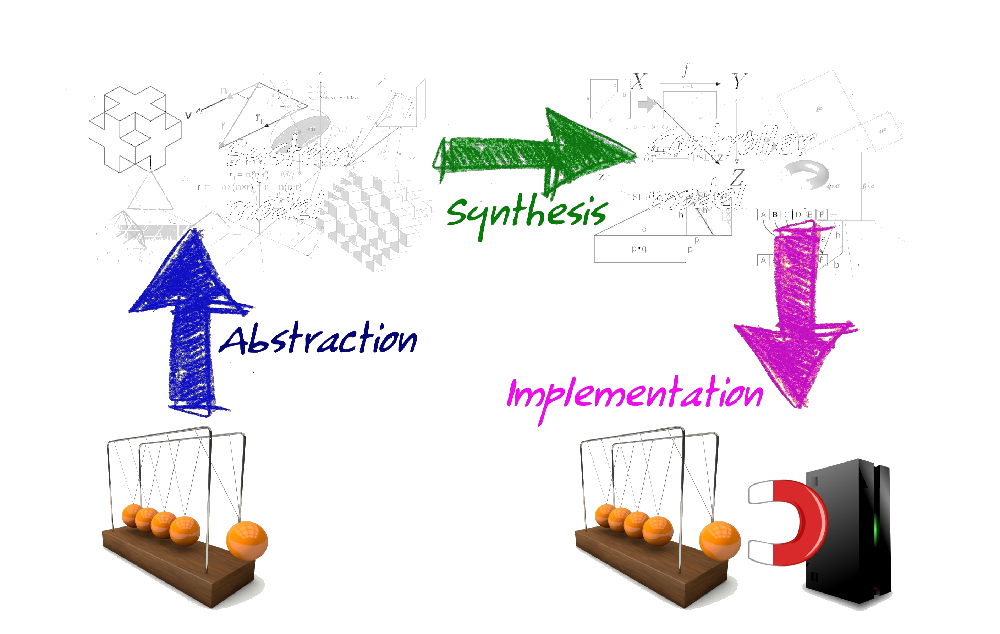
\includegraphics[width=0.85\columnwidth]{./Unit-01/img/RoleOfModels-1_cc0.png}}
  \only<3 | handout:0>{\vspace{-0.4mm}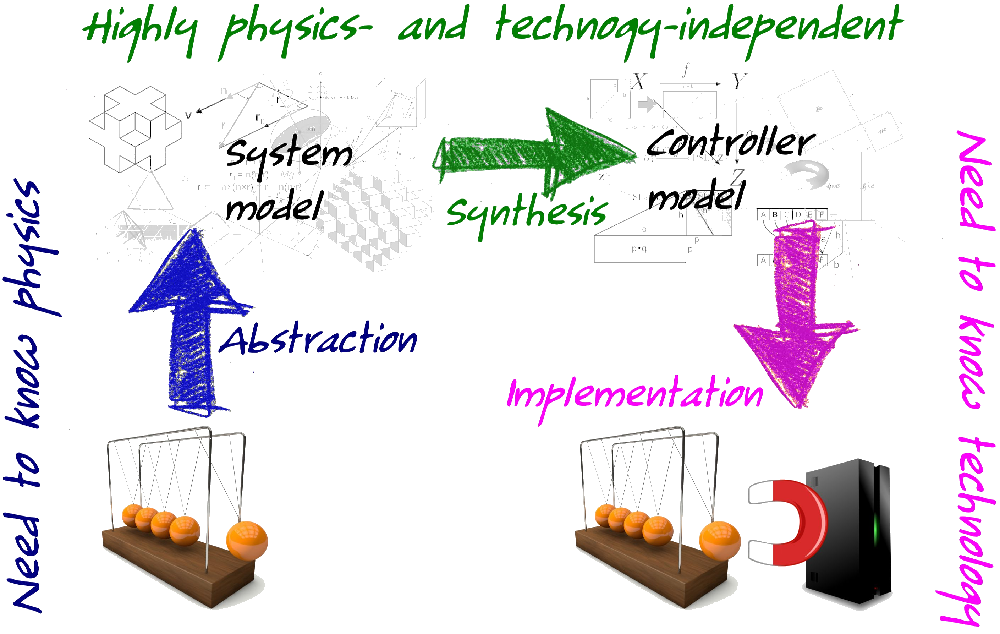
\includegraphics[width=0.85\columnwidth]{./Unit-01/img/RoleOfModels-2_cc0.png}}
  \only<4            >{\vspace{-0.4mm}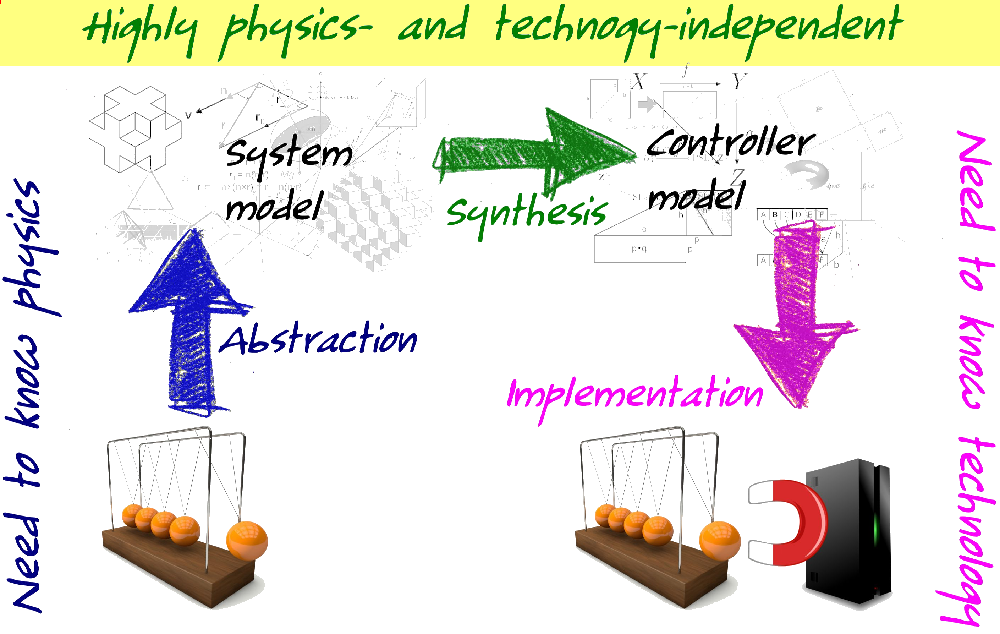
\includegraphics[width=0.85\columnwidth]{./Unit-01/img/RoleOfModels-3_cc0.png}}
 \end{center}
\end{quote}
\end{frame}

